\documentclass[a4paper,12pt]{book}
\usepackage[utf8]{inputenc}
\usepackage{graphicx}
\usepackage{titlesec}
\usepackage{hyperref}

\titleformat
{\chapter} % command
[display] % shape
{\bfseries\Huge\itshape} % format
{\small{Tic-Tac-Toe Machine Learning Workshop}} % label
{0.5ex} % sep
{
	\rule{\textwidth}{1pt}
	\vspace{1ex}
	\centering
} % before-code
[
\vspace{-0.5ex}%
\rule{\textwidth}{0.3pt}
] % after-code





% Default fixed font does not support bold face
\DeclareFixedFont{\ttb}{T1}{txtt}{bx}{n}{12} % for bold
\DeclareFixedFont{\ttm}{T1}{txtt}{m}{n}{12}  % for normal

% Custom colors
\usepackage{color}
\definecolor{deepblue}{rgb}{0,0,0.5}
\definecolor{deepred}{rgb}{0.6,0,0}
\definecolor{deepgreen}{rgb}{0,0.5,0}

\usepackage{listings}

% Python style for highlighting
\newcommand\pythonstyle{\lstset{
		language=Python,
		basicstyle=\ttm,
		otherkeywords={self},             % Add keywords here
		keywordstyle=\ttb\color{deepblue},
		emph={MyClass,__init__},          % Custom highlighting
		emphstyle=\ttb\color{deepred},    % Custom highlighting style
		stringstyle=\color{deepgreen},
		frame=tb,                         % Any extra options here
		showstringspaces=false            % 
}}


% Python environment
\lstnewenvironment{python}[1][]
{
	\pythonstyle
	\lstset{#1}
}
{}

% Python for external files
\newcommand\pythonexternal[2][]{{
		\pythonstyle
		\lstinputlisting[#1]{#2}}}

% Python for inline
\newcommand\pythoninline[1]{{\pythonstyle\lstinline!#1!}}

\begin{document}
	
	\author{Martin Mrugała\\Patryk Walczak\\Filip Szymczak\\Bartek Żyła\\Maciej Zalewski}
	\title{\Huge{\bf{Machine Learning Workshop\\Tic-Tac-Toe Project}}}
	\date{\emph{\today}}
	
	\frontmatter
	\maketitle

	\tableofcontents
	
	\mainmatter
	\chapter{Introduction}
	\section{Standard Tic-tac-toe}
	According to the definition in the Oxford Dictionary of English, Tic-tac-toe is a game in which two players seek to complete a row of either three noughts or three crosses drawn alternately in the spaces of a grid of nine squares.
		\begin{figure}[!h]
		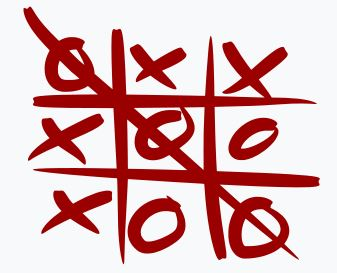
\includegraphics{./Images/1.jpg}
		\centering
		\caption{A completed game of Tic-tac-toe\protect\footnotemark.}
		\label{fig:Capture1}
	\end{figure}
	\footnotetext{Source of the image: \url{https://en.wikipedia.org/wiki/Tic-tac-toe}}
	And as it turns out, there are 255 168 possible games. So this means that, with the help of the reinforcement learning, a bot may be trained to mastery. 
	\newpage
	\section{Our implementation}
	Our team decided to create a bot which would play an expanded version of the game. The principal changes concern, inter alia:\\
	\begin{itemize}
		\item \textbf{The size of the grid could be infinite}\\
		The number of squares is not boundless, of course. Due to the CPU, as well as the storage limitations, the infinity has to be simulated. We came up with three solutions. The first one is pretty straightforward, but a little preachy. The idea is to set the size in advance. The second one, in turn, assumes an increase in the size whenever the players get close to the edge. The third one assumes that a player should not make a move which is too far from the symbols already placed on the board, as it would do very little to interfere with the other player's gameplan.
		\item \textbf{Condition of winning}\\
		The length of the sequence of X's or O's needed to win may have any value. Naturally, it has to satisfy the following condition:
		\begin{center}
			$0 < length < edgelength$
		\end{center}
		There is still the matter of the draw. In case of the constant size gird, the tie occurs whenever there is no way for any player to win.
	\end{itemize}
	\section{Machine Learning backgroud}
To deal with the problem we are using reinforcement learning, which trains algorithm by a system of reward and punishment. In this way we can match one bot against the other and let them play so that they will find the best solutions to the game by themselves without any supervision. 
\\Basic reinforcement learning can be modeled as a Markov decision process:
	\begin{itemize}
		\item set of states $S$ (state space)
		\item set of actions $A$ (action space)
		\item reward $R$ after transition from state $s$ to $s'$ under action $a$
		\item probability of transition from state $s$ to $s'$ under action $a$
	\end{itemize}
\pagebreak

\begin{figure}[!h]
	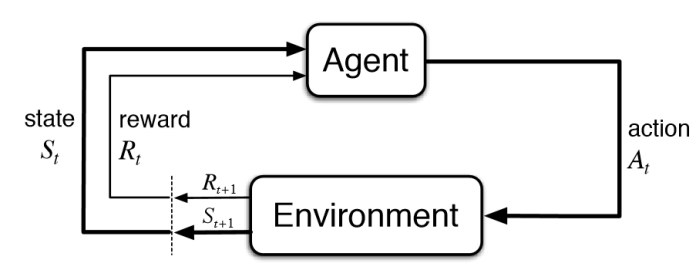
\includegraphics{./Images/RLdiag.jpg}
	\centering
	\caption{Decision process diagram\protect\footnotemark.}
	\label{fig:Capture1}
\end{figure}
\footnotetext{Source of the image: \url{https://www.kdnuggets.com/images/reinforcement-learning-fig1-700.jpg}}

A reward is a scalar feedback signal, which indicates how well the agent is doing at the given step $R_{t}$. Reinforcement is based on the reward hypothesis, which tells that goals can be described by the maximisation of expected cumulative reward, so the agent's job is to maximise cumulative reward. To do so, in our implementation, it selects actions which give the greatest reward (have the greatest value) immediately. 

Observation is the information about environment received by the agent. The history is the sequence of observations, actions and rewards up to time $t$.

\begin{equation}
	H_{t} = A_{1}, O_{1}, R_{1}, ...,  A_{t}, O_{t}, R_{t}
\end{equation}

State is the information used to determine the next action. Our environment (game board) is fully observable, so the state of the environment is the same as the state of the agent and observation of the agent. State can be described as a function of history.

\begin{equation}
	S_{t} = f(H_{t})
\end{equation}

A state $S_{t}$ is Markov state if and only if

\begin{equation}
	P[S_{t+1} | S_{t}] = P[S_{t+1} | S_{1}, ..., S_{t}]
\end{equation}

Then, if the current state is known, the history is not needed. State $S_{t}$ is enough to decide on the next action.
Additionaly, as stated earlier, our environment is fully observable, which means that the agent state is equal to the environment state; the agent has all information about environment.

Reinforcement learning agent contains two components: policy and value function. The policy describes how the agent behaves, it is a map from state to action. Value function tells how good each state or action is. 

In our implementation the policy is a dictionary containing every state encountered during learning with some value. Value function decides which move is the best by analysing these values for the next actions, but only one ahead. Our agent is using a deterministic policy, the action is chosen by finding the greatest value for the next state. There is only a slight probability for doing a random action, thanks to this the algorithm can learn and explore new paths.


	\chapter{Solution}

We have prepared two basic versions, for finite and infinite boards, and one which is doing smarter moves for the infinite board.

	\section{Finite board}
Bot algorithm is trained against the other instance of the bot at the beginning, then the winner is chosen by comparing the number of wins and forwarded to the player as the best current solution on the proper position (O or X). Iterations are the number of games to play between bots - the more they play, the better they are.
	
\begin{python}
def train(iterations):
	player1Win = 0.0
	player2Win = 0.0
	loadPolicy()
	for i in range(0, iterations):
		play()
		if (player1 wins):
			player1Win += 1
			player1.feedReward(1)
			player2.feedReward(0)
		if (player2 wins):
			player2Win += 1
			player1.feedReward(0)
			player2.feedReward(1)
		if (draw):
			player1Win += 1
			player1.feedReward(0.1)
			player2.feedReward(0.1)
	savePolicy()
	if (player1Win > player2Win):
		return player1
	else:
		return player2
\end{python}

Limiter in the bot instance limits the range of the optional moves on the board. ExploreRate is a probability of a random action, stepSize controls the increment of value for the given state during reward feeding. 

In this function, the set of actions is constructed for a given state. AI decides which move to make by considering every possibility in it's current bounds. The move is analyzed by checking how the state would look like after the action. If such situation on the board has not occured before (it is not in the estimations), the new state is given the value (1 for win, 0 for lose and 0.5 otherwise), hashed and added to the estimations dictionary.

\begin{python}
def move(state):
    nextStates[ ]
    nextPositions[ ]
      for i in range (-limiter, limiter+1):
        for j in range (-limiter, limiter+1):
          if move is possible:
            nextPositions.append((i,j))
            nextStates.append(nextState(i,j).getHash())
            if nextState(i,j).getHash() not in estimations:
            if nextState(i,j).isEnd:
              if win:
                estimations[nextState(i,j).getHash()] = 1
              else:
                estimations[nextState(i,j).getHash()] = 0
            else:
              estimations[nextState(i,j).getHash()] = 0.5
\end{python}
 
After calculations the decision has to be made. There is a chance to perform a random action (probability of this is given by exploreRate), which allows to explore new paths with a possibility of finding a new, better tactic. Otherwise the action with the biggest value based on the previous training is chosen.

\begin{python}
if random.binomial(1, exploreRate):
	r = random.(0, length(nextPositions)-1)
	action = nextPositions[r]
	states.append(nextStates[r])
	return action

values = [ ]
for hash, position in (nextStates, nextPositions):
	values.append((estimations[hash], position))
v = value.index(max(values.estimation))
action = values[v][1]
states.append(nextStates[v])
return action	
\end{python}

Upon finishing the game iteration, algorithm is fed with the reward according to the result. Values for states from the path chosen in the current iteration are adjusted starting from the last one. The change depends on the "size" of the reward, stepSize and values of previously rewarded states along the path when going back. 
That is how the algorithm learns which paths are better to choose and which ones should be rather ommited. If the outcome was positive, values will be slightly increased. If the game was lost, values will drop down a little bit. The changes are scaled so they are small and do not affect strongly the possibility of choosing other paths. Parameters can be changed to find the optimal way of learning.

\begin{python}
def feedReward(reward):
  if length(states) == 0:
    return
  target = reward
  for latestState in reversed(states):
    value = estimations[latestState] 
		+ stepSize * (target - estimations[latestState])
    estimations[latestState] = value
    target = value
\end{python}

There are two policies, optimal policy 1 is for the starting bot and optimal policy 2 is for the bot which has second move. Each training session starts with loading the last optimal policy as estimations and ends with saving them. 

The file contains hashed states, which allows for a quick comparison as keys, and their appropriate values in a dictionary. In this way we do not have to store and compare the whole state, calculating hash is enough to preserve the uniqueness of the state. Only the set of moves is being hashed, the order is not important. Stored data should be reduced to the necessary minimum because the number of possible states grows very quickly (for the infinite board there is an infinite number of states).

\begin{figure}[!h]
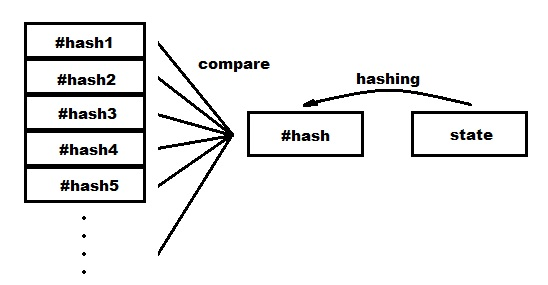
\includegraphics{./Images/hashing.jpg}
	\centering
	\caption{Comparision of a given state with the estimations.}
	\label{fig:Capture1}
\end{figure}

	\section{Infinite board}

For the infinite board the agent is the same as for the finite one. The only change is in the $move()$ function. To deal with the infinity, if there are no more possible positions in the currently considered bounded area, boundaries are extended and the process continues. This is done before choosing the next move. Bounds value is equal to the limiter starting value.

\begin{python}
def move(state):
	...

	if length(nextPositions) == 0:
		limiter += bounds
		return move(state)

	...
\end{python}

	\section{Infinite board (smarter moves)}

On the infinite board there are infinite possibilities for the next move. To help our agent in playing and in the learning process, we are limiting the set of possible actions by eliminating ones which are pointless from the logical point of view. 

To be exact, the set of possible moves consists of positions which are in the neighborhood (described by $limiter$ value here) of already taken positions. In that way we will not have situations where the bot randomly decides to make a move on some position far away from the center of the action, which is ineffective and illogical. 

Additionaly, if the bot is starting the game, the first move will be at a random position in the middle of the board (3x3 square).

\begin{python}
def move(state):
  nextStates[ ]
  nextPositions[ ]

  if length(state.data) == 0:
    i = random.randint(0,3)
    j = random.randint(0,3)
    nextPositions.append((i,j))
    nextStates.append(state.nextState(i,j).getHash())

  ...
  
  else:
    for position in state.data:
      for i in range (-limiter, limiter+1):
        for j in range (-limiter, limiter+1):
          ii = position[0] + i
          jj = position[1] + j
          if (ii,jj) not in state.data:
             nextPositions.append((ii,jj))
             nextStates.append(state.nextState(ii,jj).getHash())
  
  ...
\end{python}

	\chapter{Results}

	\section{Predictions}

As it was mentioned at the beginning, the number of possible games on the 3x3 board is 255 168. When the size increases, the number of possible games skyrockets to an unimaginably large number. It is not that hard for the algorithm to find all the possible states of the game for the fairly small boards, but every small change to the board size generates a lot of new possibilities. The minimal number for moves to win, if the winning condition is 3 in a row, is 5 and maximum is the number of positions on the board. For each number of moves we have to consider every possible state of the game. For the infinite board this number goes to infinity.

\begin{figure}[!h]
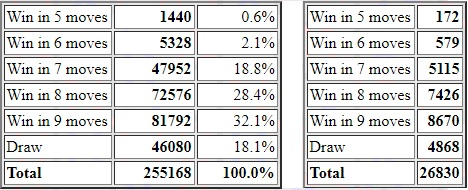
\includegraphics{./Images/3x3moves.jpg}
	\centering
	\caption{Combinations of moves for a 3x3 board\protect\footnotemark}
	\label{fig:Capture3}
\end{figure}
\footnotetext{Source of the image: \url{http://www.se16.info/hgb/tictactoe.htm}}

Theoretically our bot should be able to achive skill level which will be enough to play on a par with a human. Unfortunately, as we expected, to do so, even on a finite board, the agent should go through more iterations than we were capable of running. Policy file quickly grows to a huge size and we do not have enough computational power to train it well enough.

While it is not capable of decisively winning against a human, results of our training show that the algorithm is working correctly and we can assume that after enough iterations it should play as expected. 

This statement is based on results of two bots playing against each other and fact that the player who starts has better chances of winning in Tic-Tac-Toe, because the second one has to react to his moves. If the first one does not make any mistake in the worst scenario, on the finite board, the result of the game will be a draw. For the infinite board there are no draws, so the starting player should always win.

 	\section{Finite board}

Parameters and results for the tests:

\begin{description}
	\item 5x5
	\item iterations = 300 000
	\item boardSize = 5
	\item need for win = 4
	\item limiter = 2
	\item stepSize = 0,1
	\item exploreRate = 0,3
	\item Player1 wins = 56\%
	\item Player2 wins = 44\%
	\newline
	\item 3x3
	\item iterations = 500 000
	\item boardSize = 3
	\item need for win = 3
	\item limiter = 1
	\item stepSize = 0,1
	\item exploreRate = 0,3
	\item Player1 wins = 60\%
	\item Player2 wins = 40\%
\end{description}

Obtained results were satisfying and as expected. Both bots (trained for Player1 and Player2) were losing to a human player but their actions were not completely random. At the end of the training on a 3x3 board the number of games which were won by the bot with first move was approximately 2/3 of all played games. On the other hand after only a few thousands it was slightly more than 1/2. It shows that the algorithm works for the finite board, because the starting player has an advantage and, without any mistakes, should always win or at least have a draw. With more iterations we can expect to achieve better results, but the improvement will be slower than at the beginning.

 	\section{Infinite board}

Parameters and results for the tests:

\begin{description}
	\item iterations = 100 000
	\item need for win = 5
	\item limiter = 5
	\item stepSize = 0,1
	\item exploreRate = 0,3
	\item Player1 wins = 57\%
	\item Player2 wins = 43\%
\end{description}

This version is somewhat sluggish to train, thus we only ran 100 000 iterations. The results were not entirely satisfying. Bots were losing to a human player and their moves didn't make too much sense. The bot placed 2 symbols close to eachother without following through on them. Clearly expanding the approach from the finite version only by increasing the area for possible moves was not enough. Still, the starting bot (Player1) was better than the second one.

 	\section{Infinite board (smarter moves)}

Parameters and results for the tests:

\begin{description}
	\item iterations = 10 000 000
	\item need for win = 3
	\item limiter = 2
	\item stepSize = 0,1
	\item exploreRate = 0,3
	\item Player1 wins = 63\%
	\item Player2 wins = 37\%
\end{description}

After changes which limit the actions to the "center" of the game, results are much better. They are able to choose next moves more wisely than before. It is also easier for them to deal with the infinite possibilities of moves. With further training the first bot would continue expanding the gap in skill between the bots.

 	\section{Summary}

Our implementation of reinforcement learning to build a bot for the Tic-Tac-Toe game works quite well when it comes to playing with the other bot and meets our expectations. When playing together, the first bot is winning significantly more often. 

On the other hand playing with a human is not recommended at this moment, because bots still need more training and tests. Unfortunately, we are not able to perform such computations. To deal with this problem we could try to find more powerful computer or try to optimalise the bot further. 

Creating a bot which will be able to make decisions on the infinite board requires a lot of training iterations. Learning to play on a finite board is much faster. From possible changes, we could add choosing the best move randomly if there is more than one with the same maximum value or making the bot look through not the entire states library.

	\chapter{Instruction}

There are three versions of the program, each in their respective folder. The Player makes a move by inputting two integers, x and y, which corresponds to the x,y position in the board.

To start the training run the $game.py$ python script, at the end the results will be shown and the game will start with the better bot.

The file $game.py$ can be run with different options to have a desired result. The options are available after running $game.py --help$ and work as follows:
\begin{itemize}
	\item -i/--iterations - choose the number of iterations for the training process
	\item -t/--train - choose whether you want to train the bots (default, "y" for yes) or just play against a bot ("n" for no)
	\item -s/--start - choose whether you want to go first ("1") or second ("2") (this option only makes sense when not training, after training the better bot is chosen to play against, which usually means the first bot) 
	\item -b/--boardSize - choose the (odd) length of the side of the finite board (not implemented in the infinite case)
	\item -n/--need - the number of symbols in a row necessary to win
\end{itemize}

By default, the game is run as: $game.py$ -i 100000 -t  y -s 2 -b 3 -n 3

Important note: to play without training, policy from the previous training is needed. Otherwise the bot will not know how to play at all.

	\chapter{Bibliography}

\begin{description}
	\item Reinforcement Learning Lectures by David Silver on YouTube
	\item https://en.wikipedia.org/wiki/Reinforcement\_learning
	\item https://github.com/JaeDukSeo/reinforcement-learning-an-introduction/tree/master/chapter01
\end{description}


	\backmatter
	% bibliography, glossary and index would go here.
	
\end{document}